\documentclass[aspectratio=169]{beamer}

\usepackage[utf8]{inputenc}
\usepackage{soul}
\usepackage{pdfpcnotes}
\usepackage{listings}
\usepackage{tikz}

\usetheme{Hannover}
\usecolortheme{dove}

\AtBeginSection[]{
  \begin{frame}
  \vfill
  \centering
  \begin{beamercolorbox}[sep=8pt,center,shadow=true,rounded=true]{title}
    \usebeamerfont{title}\insertsectionhead\par%
  \end{beamercolorbox}
  \vfill
  \end{frame}
}

\lstset{language=C++,
                basicstyle=\ttfamily,
                keywordstyle=\color{blue}\ttfamily,
                stringstyle=\color{red}\ttfamily,
                commentstyle=\color{purple}\ttfamily,
                morecomment=[l][\color{magenta}]{\#}
}


\title{Eine Einführung in modernes C++ mit CMake}
\author{Paul Nykiel}
\date{\today}

\begin{document}
\maketitle
\frame{
    \tableofcontents
}

\section{Einleitung}
\begin{frame}
    \frametitle{Was ist C++}
    \pnote{Kurz Hintergrund für Einordnung}
    \begin{itemize}
        \item \st{C with classes}
            \pnote{Ursprünglicher Name, da initial nur Erweiterung von C um Objektorientung}
            \pause
        \item C++11!
            \pnote{Inzwischen weiter von C entfernt, mehr Konstrukte um sicheren und effizienten Code zu schreiben (Verweis Titel). Neuer Standard inzwischen 17 bald 20. Benennung: 98: 98 und 03. 11: 11 - 17}
            \pause
        \item Standardisiert und offen
            \pnote{Viele Compiler, Gute Dokumentation,  Entscheidungen werden im Komitee getroffen, nicht von einzelnen Firmen}
            \pause
        \item Wird in quasi jeder Domäne genutzt
            \pnote{Embedded, Betriebssysteme, Systemnahe Entwicklung, Signalverarbeitung (Codierung), Desktop-Anwendungen, Spiele, Server-Anwendungen, HPC...}
            \pause
        \item Ziele: Sicherer und performanter Code
            \pnote{Sicheres Typensystem, checks zur Compile Time (unterschied zur Run Timer hervorheben), maschinennah}
    \end{itemize}
\end{frame}

\begin{frame}
    \frametitle{C++ im Vergleich zu Java}
    \begin{itemize}
        \item Undefiniertes Verhalten 
            \pnote{Null-Pointer, fehlendes Return, division durch Null. Kann nicht vom Compiler kontrolliert werden und zur Runtime gibt es keine passnden Mechanismen  z.B. Microcontroller. Aber quasi jede Sprache hat undefiniertes Verhalten bezeichnet es aber nicht so (z.B. Race-Conditions)}
            \pause
        \item Keine automatische Speicherverwaltung 
            \pnote{Keine Aufgabe der Sprache, wenn benötigt liefert die STL passende Container. Bei Microcontroller oder Echtzeitanwendungen nicht gewünscht.
            Unterscheidung Heap und Stack hervorheben.}
            \pause
        \item Kleiner Sprachkern und kleine Standardlibrary 
            \pnote{60 Schlüsselwörter, C\# z.B. 86. Keine UI, kein Networking...}
            \pause
        \item Templates 
            \pnote{Nicht generics, viel mächtiger, z.B. Boost MSM, sichere Pointer (Guideline support library), Turing-vollständig}
            \pause
        \item Operatorenüberladung
            \pnote{Bsp. Vektor, Iteratoren...}
            \pause
        \item Tendentiell weniger tiefe Vererbung
            \pnote{Z.b. Container und Iteratoren, keine Überklasse aber Eigenschaften (forward-Iterator), dadurch weniger Boilerplate}
            \pause
        \item Mehrfachvererbung
            \pnote{Dadurch keine Interfaces notwendig, aber selten genutzt}
            \pause
        \item Definierte Objektlebenszeit
            \pnote{Konstruktor, Destruktor, Scope}
    \end{itemize}
\end{frame}

\section{Ein erstes C++ Programm}

\begin{frame}
    \Huge{Beispiel: Hello World}
    \pnote{Hello World. Erklärung: include, keine main-Klasse, namespaces, Operatorenüberladung, Vergleich Code-Länge mit Java}
\end{frame}

\begin{frame}
    \frametitle{Vom Sourcecode zur ausführbaren Datei}
    \begin{itemize}
        \item Präprozessor 
            \pnote{Erklärung include und define an Hello World Bsp (gcc -E), einfache Textersetzung, Erklärung an Tafel}
            \pause
        \item C++-Compiler 
            \pnote{Übersetzten von der Übersetzungseinheit in Maschinencode, Übersetzungseinheit definieren}
            \pause
        \item Linker 
            \pnote{Baut Programm zusammen und sucht Funktionen in anderen Übersetzungseinheiten}
            \pause
        \item includes sichern Typkonsitenz
            \pnote{Unterschied Definition und Deklaration, Doku im Header gut für Übersicht}
            \pause
        \item Templates müssen im Header definiert werden
            \pnote{Compiler muss alle instanziierungen kennen, langsamer Buildprozess}
    \end{itemize}
\end{frame}

\begin{frame}
    \Huge{Beispiel: Eine zweite Übersetzungseinheit}
    \pnote{Zweites Cpp File, alles einfach in g++ schmeißen,
    Message als std::string (nicht ref)}
\end{frame}

\section{CMake}

\begin{frame}
    \frametitle{Warum CMake}
    \begin{itemize}
        \item Nur geänderte Dateien neu kompilieren 
            \pnote{erkennt welche Files geändert wurde, größere Projekte kompilieren sonst jedes mal mehrere Minuten bis Stunden}
            \pause
        \item Einzelner Befehl an Compiler wird zu kompliziert
            \pnote{Vor allem bei vielen Flags und vielen Dateien}
            \pause
        \item Portabilität
            \pnote{Compiler und Flags werden unnabhängig vom Os und von installierten Compilern angegeben}
    \end{itemize}
\end{frame}

\begin{frame}
    \Huge{Beispiel: CMake}
    \pnote{Einfaches CMake File dazu bauen, nochmal kompilieren, Lib ändern zeigen dass main nicht neu gebaut wird}
\end{frame}

\section{Mehr C++}

\begin{frame}
    \frametitle{Speicherverwaltung}
    \begin{itemize}
        \item \lstinputlisting{examples/slides/copy.cpp}
            \pnote{f ist Funktion list->list und b ist list. Was passiert hier, wie viele Objekte existieren, wie viel Speicher wird genutzt, wie oft wird kopiert}
            \pause
        \item Jegliche Zuweisung ist eine Kopie, auch für Funktionsargumente
            \pnote{Funktionsargumente, Zuweisung.... Explizit große Container erwähnen}
            \pause
        \item Einfach verständlich
            \pnote{Vgl. komisches Java Verhalten. Trivial ein Objekt zu kopieren, deep copy in Java und C\# schwierig (Internet: selber implementieren oder serializieren und deserializieren)}
            \pause
        \item Für große Objekte unnötige Performanceeinbuße
            \pnote{Spricht gegen das was ich in Einleitung gesagt habe, Performance in C++ wichtig}
    \end{itemize}
\end{frame}

\begin{frame}
    \frametitle{Pointer}
    \begin{itemize}
        \item Pointer 
            \pnote{"Vererbt" von C}
            \pause
        \item Angst!
            \pause
        \item Gefährlich!
            \pause
        \item Böse!
            \pnote{Pointer kurz erklären, kurz Owner (malloc/new) bzw. nur als Referenz erklären}
            \pause
        \item Nicht schlimm aber viel Fehlerpotential
            \pnote{Leaks, Owner nicht definiert, vor allem bei Librarys relevant}
            \pause
        \item \lstinline{int b = 17; int *a = &b;}
            \pnote{Pointer als Referenz}
            \pause
        \item \lstinline{int *c = new int();}
            \pnote{Pointer als Owner, Hier gleich ein potentieller Leak}
            \pause
        \item \lstinline{delete c;}
            \pnote{Immer mit delete, das will doch wirklich keiner}
            \pause
        \item Gehört nicht in die Anwendungslogik
            \pnote{Permanente Fehlerquelle, Zeitverschwendung, Ab jetzt als Raw-Pointer bezeichnet und nie wieder verwenden!}
    \end{itemize}
\end{frame}

\begin{frame}
    \frametitle{Stack und Heap}
    \begin{columns}
        \begin{column}{.5\textwidth}
            \begin{itemize}
                \item Hauptspeicher (RAM) wird aus zwei Richtungen vergeben
                    \pnote{Aufteilung in Stack für Performance und Heap für dynamischen Speicher}
                \item Stack wird für Funktion aufgebaut
                    \pnote{Schnell da FILO, wird automatisch wieder abgebaut}
                \item Heap für dynamischen Speicher
                    \pnote{Langsam, freier Speicher muss erst gefunden werden}
                \item Speicher auf dem Heap muss händisch reserviert und freigegeben werden
                    \pnote{Memory Leak wenn nicht wieder freigegeben}
                \item Bei mehr als einem Owner Verwaltung kompliziert
                    \pnote{Owner: Funktion die Pointer kennt}
            \end{itemize}
        \end{column}
        \begin{column}{.5\textwidth}
            \begin{figure}[H]
                \centering
                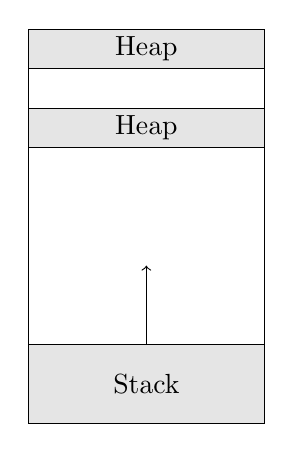
\begin{tikzpicture}
                    \draw [draw] (0,0) rectangle (3,5);
                    \filldraw [draw=black,fill=gray!20] (0,0) rectangle (3,1) node[pos=.5] {Stack};
                    \filldraw [draw=black,fill=gray!20] (0,4.5) rectangle (3,5) node[pos=.5] {Heap};
                    \filldraw [draw=black,fill=gray!20] (0,3.5) rectangle (3,4) node[pos=.5] {Heap};
                    \draw [->] (1.5,1) -- (1.5,2);
                \end{tikzpicture}
            \end{figure}
        \end{column}
    \end{columns}
\end{frame}

\begin{frame}
    \frametitle{Smart-Pointer}
    \begin{itemize}
        \item Funktionen aus der Standardlibrary
            \pnote{Erwähnung Operatorenüberladung und Lifetime}
            \pause
        \item unique\_ptr 
            \pnote{Quasi Drop-In-Replacement für Raw-Ptr, machen selber den Speicher am Ende der Lebenszeit Frei}
            \pause
        \item Genau ein Owner
            \pnote{Explizit verboten zu kopieren (=delete), Bsp. kopieren in Klasse, jetzt uneindeutiger Owner. Oftmals für Factory Methoden, kein Overhead zu Raw-Pointer}
            \pause
        \item
            \lstinline{std::unique\_ptr<int> a = std::make\_unique<int>(17);}
            \pause
        \item shared\_ptr 
            \pnote{Zusätzlich Zählen von Instanzen (siehe Copy-Constructor)}
            \pause
        \item Quasi immer nutzbar
            \pnote{Dafür kopieren... minimal langsamer (nicht bei Zugriff)}
        \item
            \lstinline{std::shared\_ptr<int> a = std::make\_shared<int>(17);}
    \end{itemize}
\end{frame}

\begin{frame}
    \frametitle{Referenzen}
    \begin{itemize}
        \item Sprachfeature kein Library-Feature
            \pnote{Werden vom Compiler zu Pointern gemacht, nie Owner. Hier betrachtet L-Value-Referenzen}
            \pause
        \item Können nicht null sein
            \pnote{Zeigen immer auf anderes Objekt, eine Art Alias}
            \pause
        \item Können aber ungültig werden
            \pnote{z.B. lokale Variablen}
            \pause
        \item
            \lstinline{int b = 17; int &a = b;}
    \end{itemize}
\end{frame}

\begin{frame}
    \frametitle{Zusammenfassung Pointer}
    \begin{itemize}
        \item Raw-Pointer: Wird quasi nie verwendet
            \pnote{Ausser pre C++11 und mit C APIs}
            \pause
        \item Unique-Pointer: Ersatz für Raw-Pointer
            \pnote{Limitierung: Ein Owner kein Overhead}
            \pause
        \item Shared-Pointer: Sichere Pointer für beliebig viele Ownerr
            \pnote{Am Ähnlichsten zu Java, aber etwas Overhead (immer noch weniger als Java und definierte Lifetime)}
            \pause
        \item Referenzen: Oftmals um Kopien zu vermeiden
            \pnote{Sprachfeature}
    \end{itemize}
\end{frame}

\begin{frame}
    \Huge{Beispiel: Pointer \& Referenzen}
    \pnote{Wo Pointer/Ref einbauen? Frage welche Sorte Pointer. HelloWorld Lib Ergänzen mit Referenzen, jetzt in CLion}
\end{frame}

\section{Design Pattern}

\begin{frame}
    \frametitle{Const-Correctness}
    \begin{itemize}
        \item Alles per Referenz: Super Effizient aber Fehlerquelle
            \pnote{Beispiel: ausversehen einfügen in Map, allgemeine Fehlerquelle immer nur minimale Rechte}
            \pause
        \item Const-Referenzen
            \pnote{Ergänze Beispiel}
            \pause
        \item \lstinline{const int &a = b;}
            \pnote{Read-Only "nur anschauen"}
            \pause
        \item Const-Memberfunktionen
            \pnote{Beispiel getter}
            \pause
        \item \lstinline{int getX() const \{...}
            \pnote{Const am ende der Definition this ist in der Funktion konstant}
            \pause
        \item Mutable
            \pnote{Beispiel Mutex, Caching, nicht immer!}
    \end{itemize}
\end{frame}

\begin{frame}
    \Huge{Beispiel: Const-Correctness}
    \pnote{const einfügen hello world}
\end{frame}

\begin{frame}
    \frametitle{RAII}
    \begin{itemize}
        \item Resource acquisition is initialization
            \pnote{Fehlerreduktion, Einfachheit}
            \pause
        \item Objekt akquiriert Resourcen im Konstruktor und gibt sie im
            Destruktor frei
            \pnote{Bsp. Datei, Mutex, Vector. Vgl try catch finally java}
            \pause
        \item
            \lstinputlisting{examples/slides/raii.cpp}
            \pnote{Trailing return type, Const-Correctness, Objekte werden im Konstruktor initialisiert, alle Objekte werden im Konstruktor geschlossen} 
    \end{itemize}
\end{frame}

\section{OOP in C++}

\begin{frame}
    \frametitle{Klassendeklaration}
    \lstinputlisting{examples/slides/class.h}
    \pnote{Hinweis unterschied Deklaration und Definition. Vererbung, Sichtbarkeit von Vererbung, public, private, Konstruktor, Trailing return type, const Const-Correctness}
\end{frame}

\begin{frame}
    \frametitle{Klassendefinition}
    \lstinputlisting{examples/slides/class.cpp}
    \pnote{Initializierung in Braced-Initializer, Super-Konstruktor, this als Pointer}
\end{frame}

\begin{frame}
    \Huge{Beispiel: HelloWorld OOP}
\end{frame}

\section{Noch mehr C++}

\begin{frame}
    \frametitle{Casts und Null-Pointer}
    \begin{itemize}
        \item \lstinline{static\_cast<T>(a)}
            \pnote{Castet Typen in kompatible Typen (hier von a nach T), kompatibilität wird zur Compile Time gecheckt}
            \pause
        \item \lstinline{dynamic\_cast<T>(a)}
            \pnote{Castet zur Runtime, vor allem für Pointer und Polyphormismus, kann Null sein}
            \pause
        \item \lstinline{0}, \lstinline{NULL} und \lstinline{nullptr}
            \pnote{Abstammung aus C, Erklärung mit Überladung}
    \end{itemize}
\end{frame}

\begin{frame}
    \frametitle{Type-Deduction}
    \lstinputlisting{examples/slides/typededuction.cpp}
    \pnote{Typ wird hergeleitet, oftmals Praktisch (vgl. Iterator), spart redundanz. Potentielle Fehlerquelle, z.B. Proxy klasse (vgl. std::vector<bool>)}
\end{frame}

\begin{frame}
    \frametitle{Kurzeinführung Templates als Generics}
    \lstinputlisting{examples/slides/template.cpp}
    \pnote{Definition von template mit Typen, Type Deduktion}
\end{frame}

\section{STL}

\begin{frame}
    \frametitle{STL}
    \begin{itemize}
        \item Standard Template Library
            \pnote{Standardlibrary, wird von der libc zur Verfügung gestellt, nicht immer existent z.B. MC, aber mit OS schon. Grob Aufteilung:}
            \pause
        \item Utility
            \pnote{String, Math, Date \& Time, Smart Pointer}
            \pause
        \item Container
            \pnote{Strukturierte Sammlung von Objekten}
            \pause
        \item Algorithmen
            \pnote{Standardalgorithmen oftmals mit Containern}
            \pause
        \item IO
            \pnote{Standard-IO, Dateizugriff}
            \pause
        \item Concurrency
            \pnote{Threads und Locking Mechanismen}
    \end{itemize}
    \pnote{Jeweils kleine Auswahl zeigen}
\end{frame}

\begin{frame}
    \frametitle{Utility}
    \begin{itemize}
        \item \lstinline{std::string}
            \pnote{Wie in Java}
            \pause
        \item \lstinline{std::unique\_ptr<T>}
            \pnote{Siehe oben}
            \pause
        \item \lstinline{std::shared\_ptr<T>}
            \pnote{Siehe oben}
            \pause
        \item \lstinline{std::chrono}
            \pnote{Nur der Namespace, diverseste Funktionen}
            \pause
        \item \lstinline{std::sin()} \ldots
            \pnote{Auch exotisches wie Riemann-Zeta Funktion}
            \pause
        \item \lstinline{std::complex} \ldots
            \pnote{Komplexe Zahlen und Hilfsfunktionen}
            \pause
        \item \lstinline{std::normal\_distribution} \ldots
            \pnote{Diverse Verteilungen und RNGs}
            \pause
        \item \lstinline{std::function<T(A...)>}
            \pnote{Behandlung von Callable (Funktionen) wie Variablen (vgl. Funktionspointer)}
    \end{itemize}
\end{frame}

\begin{frame}
    \frametitle{Container}
    \begin{itemize}
        \item \lstinline{std::array<T, N>}
            \pnote{Größe muss zu Compile-Time feststehen, wie Array in C nur Sicher, Zugriff O(1), Einfügen unmöglich}
            \pause
        \item \lstinline{std::vector<T>}
            \pnote{Dynamisch angelegtes Array, Elemente können hinzugefügt werden aber nicht effizient, Zugriff O(1), Einfügen worst case O(n)}
            \pause
        \item \lstinline{std::deque<T>}
            \pnote{Verlinkte Array-Liste, Ausprache!, Zugriff O(1) (aber langsamer als vector), Einfügen an einem Ende O(1), Einfügen in der Mitte O(n)}
            \pause
        \item \lstinline{std::list<T>} und \lstinline{std::forward\_list<T>}
            \pnote{Einfach bzw. doppelt verkettete Liste, Zugriff O(1), Einfügen O(1)}
            \pause
        \item \lstinline{std::set<T>} und \lstinline{std::map<K, V>}
            \pnote{Menge und Abbildung von Key auf Value, finden von Elementen in O(log(n(), einfügen in O(log(n))}
            \pause
        \item \lstinline{std::tuple<T...>} und \lstinline{std::pair<T1, T2>}
            \pnote{Genau genommen kein Container, Sammlung von mehreren bzw. 2 Objekten von unterschiedlichem Typ. Typen und Anzahl müssen zu Compile-Time bekannt sein}
            \pause
        \item \lstinline{std::optional<T>}
            \pnote{Variable vom Typ T die nicht existieren muss, zum Beispiel als Return-Wert mit Fehler}
    \end{itemize}
\end{frame}

\begin{frame}
    \frametitle{Iteratoren}
    \lstinputlisting{examples/slides/iterator.cpp}
    \pnote{Type deduction wäre möglich (auto). Wie Pointer nur abstrakt, z.B. auch bei Liste, zentrales Element für Container und Algorithmen,
    abstraktion von Container, wieso nicht at O(n) in Liste}
\end{frame}

\begin{frame}
    \frametitle{for-each}
    \lstinputlisting{examples/slides/foreach.cpp}
    \pnote{Deutlich kürzer, sicher beachte const Referenz, nur wenn Funktionen const}
\end{frame}

\begin{frame}
    \frametitle{Concurrency}
    \begin{itemize}
        \item \lstinline{std::thread}
            \pnote{Startet neuen Thread aus callable}
            \pause
        \item \lstinline{std::launch} und \lstinline{std::future<T>}
            \pnote{Abstraktion, asynchroner Funktionsaufruf. Ergebnis in std::future}
            \pause
        \item \lstinline{std::mutex} und \lstinline{std::lock\_guard<T>}
            \pnote{Gegenseitiger Ausschluss. lock_guard sperrt und entsperrt automatisch (RAII!)}
            \pause
        \item \lstinline{std::atomic<T>}
            \pnote{Effiziente und kompakte Lösung für einzelne Variablen, auf denen Operationen Atomar sein sollen}
    \end{itemize}
\end{frame}

\section{Praxis}
\begin{frame}
    \Huge{Praxis: \pause Huffman-Codierer}
    \pnote{Begründung: Baum nicht als STL-Datenstrukur, trotzdem STL Container notwendig, Templates, Pointer, in unter 150 Zeilen lösbar}
\end{frame}

\begin{frame}
    \frametitle{Vorgehen}
    \begin{itemize}
        \item Datei einlesen
            \pnote{Streams nutzen}
            \pause
        \item Relative Häufigkeiten ($\approx$ Wahrscheinlichkeiten) berechnen (Byteweise)
            \pnote{Blockgröße 8-bit}
            \pause
        \item Huffman-Baum konstruieren
            \pause
            \pnote{Erstmal separate Template-Klasse für Baum, dann nutzen für Huffman}
            \begin{itemize}
                \item Menge aller Symbole mit zugehörigen Wahrscheinlichkeiten
                    \pnote{Nach passender Datenstruktur für Menge und Symbol mit Wahrscheinlichkeit fragen}
                    \pause
                \item Zwei Symbole geringster Wahrscheinlichkeit finden
                    \pnote{Effizienz, jedes mal suchen, ein mal sortieren?}
                    \pause
                \item Symbole aus Menge Entfernen
                    \pnote{Recherche wie in STL möglich}
                    \pause
                \item Zu neuem Knoten kombinieren
                    \pause
                \item Knoten zu Menge hinzufügen
                    \pause
            \end{itemize}
        \item Abbildung ausgeben
            \pnote{Durch Baum laufen, nach Format a -> 001}
            \pnote{Beispiel an Tafel!}
    \end{itemize}
\end{frame}

\section{Tools}
\pnote{Kleine Auswahl an Tools}
\begin{frame}
    \frametitle{GTest}
    \lstinputlisting{examples/slides/gtest.cpp}
    \pnote{Diverseste Bedinungen, z.B. auch Float, integration in CLion}
\end{frame}

\begin{frame}
    \frametitle{Debugging und Fehlersuche}
    \begin{itemize}
        \item Debugger
            \pnote{z.B. GDB, quasi beliebig, wichtigestes Tool}
            \pause
        \item Valgrind
            \pnote{Erkennt Speicherlecks, undefiniertes Verhalten, aber Langsam}
            \pause
        \item LibAdressSanitizer (Asan)
            \pnote{Wie Valgrind nur schnell und neuer}
            \pause
        \item clang-tidy
            \pnote{Statische Analyse, Fehler vor der Compilieren entdecken}
    \end{itemize}
\end{frame}

\section{Abschluss}

\begin{frame}
    \frametitle{Was fehlt?}
    \begin{itemize}
        \item R-Value Referenzen, forward/universal Referenzen
            \pnote{Neue Form von Referenz (ab C++11), primär benötigt wenn nicht triviale Speicherverwaltung}
            \pause
        \item Move
            \pnote{Speicher von einer Klasse an eine andere Übergeben, z.B. return, per default da, sonst wenn nicht triviale Speicherverwaltung}
            \pause
        \item Destruktor und Copy / Move Konstruktor
            \pnote{Wird per default angelegt, muss nur angelegt werden wenn nicht trivialer Speicher verwaltet wird}
            \pause
        \item Operatorenüberladung
            \pnote{Nur spezielle Member Funktionen, einfach!}
            \pause
        \item Friend Definition
            \pnote{Wird selten benötigt, einfach einzulesen}
            \pause
        \item Meta-Programming
            \pnote{Touring-vollständige Sprache zur CompileTime, type\_traits, bringt zwar Vorteile aber nicht notwendig}
    \end{itemize}
\end{frame}

\begin{frame}
    \frametitle{Mehr Informationen}
    \begin{itemize}
        \item en.cppreference.com
            \pnote{Dokumentation der Sprache und STL, deutsche Version ist Shit}
            \pause
        \item github.com/isocpp/CppCoreGuidelines
            \pnote{Gut für Designentscheidungen}
            \pause
        \item godbolt.org
            \pnote{Was erzeugt der Compiler für Code auf unterschiedlichen Plattformen, eher als Spielzeug}
            \pause
        \item github.com/SoPra-Team-10/CppCMakeIntro
            \pnote{Dieser Vortrag}
            \pause
        \item Scott Meyers: Effective Modern C++
            \pnote{Gutes Buch, deutliche Vertiefung}
    \end{itemize}
\end{frame}

\end{document}
